% !TEX encoding = UTF-8
% !TEX TS-program = pdflatex
% !TEX root = ../tesi.tex

%**************************************************************
\chapter{Finalità del mio stage in Siav}
\label{cap:process-mining}
%**************************************************************
\section{Le possibilità offerte dallo stage}
%**************************************************************
\subsection{Nuovi concetti}
Sono venuto a conoscenza della proposta di stage da parte di Siav attraverso l'evento Stage-IT. Inizialmente l'ho scartata a causa della descrizione fin troppo generica degli argomenti di stage. Successivamente, tramite contatto diretto con il responsabile, ho avuto modo di cambiare idea. Una volta chiarite le finalità delle proposte di stage, ho compreso la congenialità alla mia indole. Dalla prospettiva di realizzare un applicativo web, mi si aprivano contemporaneamente due nuove possibilità: Conoscere alcuni concetti di \textit{process mining} e alcune tecnologie front-end.


Le proposte disponibili erano 2:
\begin{itemize}
    \item La realizzazione di una \textit{fork} di una libreria per la creazione di grafi esplorabili per integrare delle funzionalità congeniali alla rappresentazione dei processi; 
    \item Lo studio dell'\acrshort{ux}\glsfirstoccur per la gestione e inserimento dei \acrshort{kpi} da concretizzare in un interfaccia utente.
\end{itemize}

Ho capito subito che la seconda proposta era quella che comportava maggiore studio teorico dell'argomento trattato e perciò l'ho scelta come preferenza comunicandola al responsabile. Nella mia scelta è stata determinante l'origine del contenuto: argomenti a me sconosciuti e perciò molto più stimolanti rispetto alla grafica vettoriale su cui ho già avuto qualche esperienza per diletto.
%**************************************************************
\subsection{Libertà di apprendere}
Un altro dei fattori che mi hanno permesso di scegliere è, sicuramente, il contesto aziendale.
Lavorare all'interno di un azienda strutturata all'interno del reparto \acrshort{rnd} ha comportato allo stesso tempo, responsabilità e opportunità.
Responsabilità perché, nello studiare l'\acrshort{ux} per la divisione ricerca e sviluppo di un ambiente professionale, c'è la necessità di non essere mai banale e di dare il massimo per ottenere poco ovvero di vagliare a lungo molte strade e scenari anche per una sola minima funzionalità.
L'opportunità è invece quella di confrontarsi con professionisti mantenendo però un certo grado di libertà di effettuare, a valle dello studio, diverse prove, proposte e infine decisioni. Il tutto condito dalla filosofia del non prendere ogni indicazione come assoluto ma discutere insieme le proposte.

Nel periodo iniziale ho dovuto affrontare diverse formazioni, alcune in maniera autonoma, altre guidate dal mio tutor che mi ha introdotto ai concetti fondamentali con formazioni teoriche e pratiche sull'argomento.
Ciononostante, durante il percorso sono insorte diverse lacune essendo il \textit{process mining} un argomento comunque troppo esteso per poter vantare un bagaglio completo di competenze durante le 320 ore previste. Fortunatamente, lavorando a diretto contatto con il tutor aziendale, ho avuto la possibilità di colmare rapidamente tali mancanze.

%**************************************************************
\section{Principi di Process Mining}
%**************************************************************
\subsection{La gestione dei processi aziendali}

La misura di un indice di processo può risultare un attività semplice per un umano, come per esempio contare il numero di pratiche da gestire rimanenti o contare gli slot per bancali disponibili all'interno di un magazzino, ma può diventare un attività assai onerosa come calcolare la liquidità disponibile controllando quali fatture verranno pagate nei prossimi trenta giorni o misurare il tempo medio di gestione di una pratica dal momento in cui viene sottoposta a quello in cui viene evasa.

La gestione complica ulteriormente le cose: la mia azienda impiega 2 giorni e 14 ore, dalla ricezione, per evadere una pratica. Per ridurre tale tempo, ho bisogno di effettuare delle prove per vedere quale sia il problema o affidarmi ad una consulenza esterna.
Come anticipato in \S\ref{subsec:occupazioneRnd}, l'esigenza di monitorare e gestire i processi aziendali, per Siav, ha origine nella digitalizzazione dei processi: una volta che essi sono digitali, risulta più facile e istantaneo, monitorarli tramite tecniche di \textit{process mining}.

Includendo Bipod all'interno dei prodotti offerti, le potenzialità della gamma software Siav, si estendono ulteriormente.
Il monitoraggio risulta istantaneo e, tramite una configurazione della piattaforma ad-hoc, l'individuazione di problemi come eccedenze, carenze, ritardi o colli di bottiglia, è un operazione veloce. Sottraendo tempo all'individuazione dei problemi, se ne guadagna ulteriore per ricercare ed effettuare delle migliorie, arrivando a lavorare con maggiore qualità.

%**************************************************************
\subsection{Da dato ad informazione}
\begin{figure}[H]
    \centering
    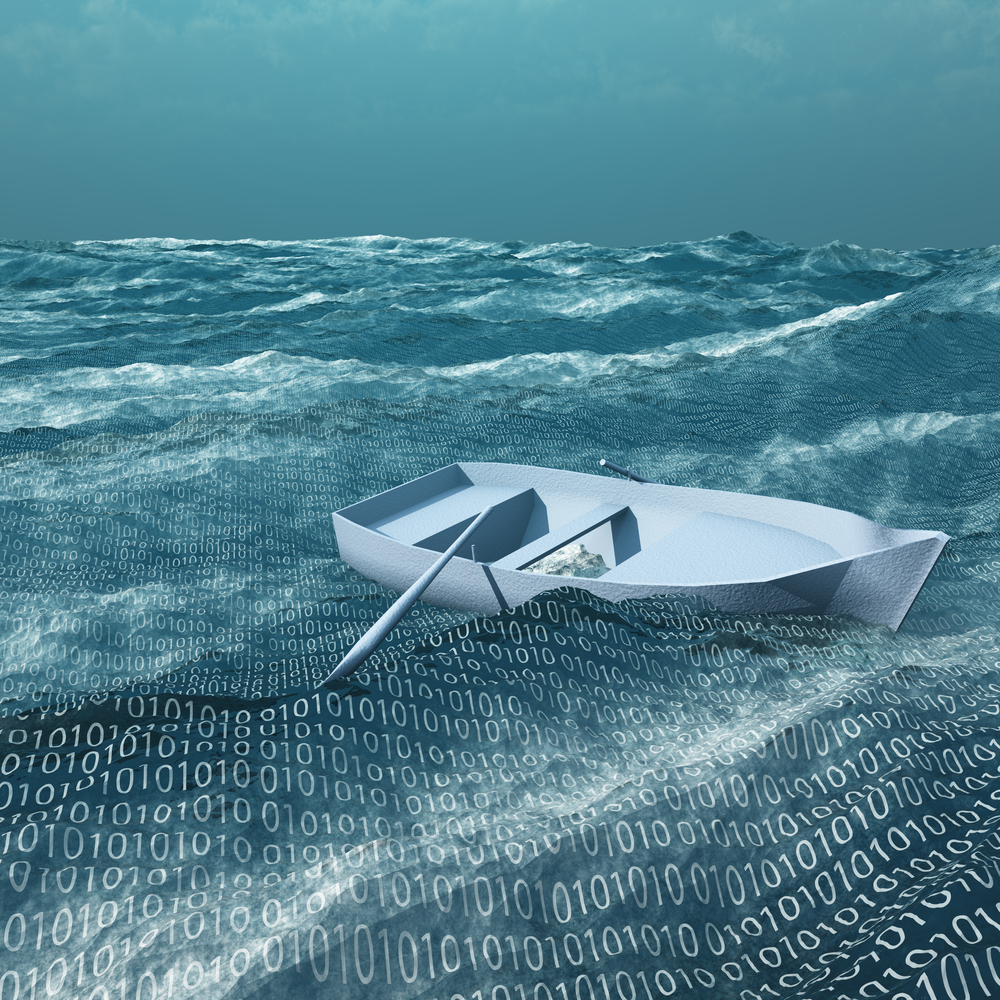
\includegraphics[width=0.50\columnwidth]{immagini/bigData.jpg}
    \caption{\textit{Data Sea} - Fonte: \href{https://www.klick.com/health/news/blog/strategy/is-medium-data-better-than-big-data/}{IS MEDIUM DATA BETTER THAN BIG DATA? - klick}}
    \label{fig:my_label}
\end{figure}

Una conseguenza della digitalizzazione dei processi è un sensibile aumento del quantitativo di dati digitali presenti e circolanti all'interno di un organizzazione. Metaforicamente lo definisco come un mare di bit di contenuto più o meno informativo da cui pescare le informazioni. L'operazione fondamentale per recuperare i pesci che ci interessano è scindere il dato utile da quello meno sfruttando uno strumento di "filtraggio".
La tipologia della rete, per granularità e dimensione, usata per pescare è discriminante fondamentale per ottenere la specie ittica desiderata.
\subsubsection{Termini}
In \textit{process mining} quella rete viene definita come \emph{termine} e gli elementi che lo caratterizzano sono i seguenti:
\paragraph{Cosa}
I dati raggruppati da un termine vengono selezionati tramite diversi filtri che possono venire applicati al contenuto o a proprietà che i dati possiedono;

\paragraph{Dove}
I dati che concorrono a rientrare in un termine, possono essere distinti tramite un processo di riferimento. Esso ne discrimina la provenienza ed è utile perciò per individuarli in maniera corretta .

\paragraph{Come}
Il termine può interpretare in diverse maniere i dati che lo compongono come per esempio:
\begin{itemize}
    \item Calcolare la durata media di un processo
    \item Calcolare quante volte un processo è stato eseguito
    \item Calcolare la somma o la media di una proprietà di tutte le esecuzioni di un processo
    \item Calcolare la durata di un evento all'interno di un esecuzione
    \item Calcolare la somma o la media di una proprietà all'interno di un evento
\end{itemize}

\paragraph{Quando}
I dati possono essere filtrati temporalmente, definendo un range entro il quale essi siano accettabili. Così facendo, posso per esempio ottenere facilmente lo stesso set di dati ma relativo a due periodi differenti.
\subsubsection{Kpi}
Un termine raggruppa tutti i dati della stessa specie sotto un unico nome.
Le operazioni sopra descritte per individuare correttamente un termine non sempre sono sufficienti per renderlo utile. La trasformazione in informazione avviene solo attraverso l'interpretazione e la correlazione con altri dati.

Lo strumento che ci permette di fare ciò viene detto \acrshort{kpi}. Il \acrlong{kpi} ci fornisce un idea qualitativa dell'andamento di un aspetto di un processo combinando e confrontando diversi dati.
Questo perché il suo calcolo è frutto di operazioni fra dati o termini e raffronto con altri dati o valori.
Per un \acrshort{kpi} posso definire delle \emph{soglie} che ne determinino uno stato ovvero quanto l'informazione che il kpi rappresenta sia piacevole o meno.
\begin{figure}[H]
    \centering
    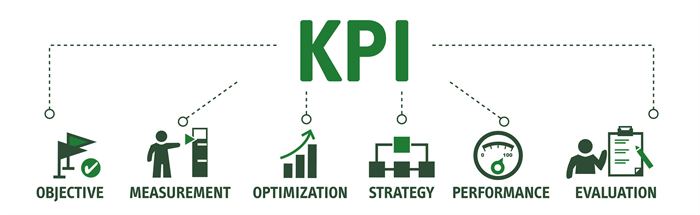
\includegraphics[width=0.80\columnwidth]{immagini/kpi.png}
    \caption{Kpi - Fonte: \href{https://incarnato.consulting/kpi-cosa-utilizzarli-nella-tua-impresa/}{KPI - Incarnato Consulting}}
    \label{fig:my_label}
\end{figure}
%**************************************************************
\subsection{KPI e \textit{dashboards} nel process mining}
Lo scopo di un cruscotto informativo all'interno di un automezzo è quello di informare il conducente, in maniera chiara e lampante, riguardo a diverse informazioni importanti relative a ciò che sta guidando come per esempio la velocità, i giri di funzionamento del motore o l'ottimalità del livello dell'olio. Questo perché la prerogativa dell'attività di guidare è quella di portare il mezzo a destinazione stando attento a rispettare vincoli e segnali, non quella di essere un attento meccanico che ha bisogno di fermarsi ogni cento metri per controllare il livello dell'olio o verificare quanto tempo ha impiegato a percorrerli. Alla stessa maniera, la persona che si trova a condurre un azienda o essere responsabile dell'andamento di un processo ha come unico scopo tale attività. Una volta individuate le informazioni di cui egli ha bisogno, è necessario evidenziare l'andamento positivo o negativo delle sole informazioni utili alla sua attività raccogliendole all'interno di un pannello chiamato \textit{dashboard}.

Le \textit{dashboards} o cruscotti, sono uno strumento informativo che evidenzia in maniera facilmente fruibile un informazione in base alla sua natura. Questa evidenziazione può essere effettuata tramite componenti grafiche di diverso genere come \textit{gauge} o istogrammi o tramite la visualizzazione di valori informativi che possono esprimere significato  anche tramite la presentazione (ad esempio sfruttando i colori di un semaforo che, per intuito collettivo, suggeriscono degli stati).
Tali componenti devono essere organizzate spazialmente a seconda dell'importanza per dare il giusto peso ad ognuno.
\begin{figure}[H]
    \centering
    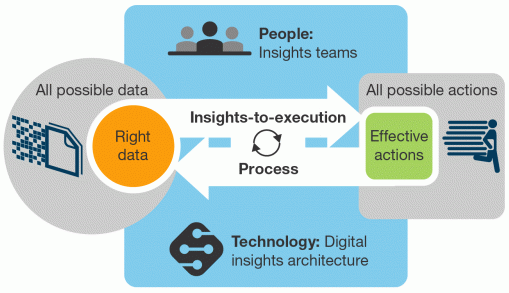
\includegraphics[width=0.80\columnwidth]{immagini/from_data_to_insight.png}
    \caption{\textit{From data to actions} - Fonte: \href{https://go.forrester.com/blogs/15-04-27-digital_insights_are_the_new_currency_of_business/}{Digital Insights Are the New Currency of Business - Forrester}}
    \label{fig:my_label}
\end{figure}
%**************************************************************
\subsection{I ruoli nella gestione e amministrazione di processo}
I soggetti che partecipano all'attività di gestione e amministrazione di processo sono fondamentalmente 2:
\begin{itemize}
    \item Il consulente ovvero colui che configura la piattaforma per mettere in rilevazione correttamente i \acrshort{kpi}. Di conseguenza detiene l'oneroso compito di comprendere le esigenze del destinatario della sua consulenza, compito che trova l'implementazione finale nella configurazione della dashboard;
    \item L'amministratore, l'utente che utilizza la dashboard per monitorare i processi e avviare gli interventi in caso di necessità.
\end{itemize}
Sono due ruoli con competenze e background differenti ma che necessitano di comunicare con un linguaggio comune e immediato
%**************************************************************
\subsection{Le esigenze degli utenti}
\subsubsection{Inserimento e gestione Kpi}
Il consulente che si appresta ad effettuare una configurazione per il suo mandante, deve conoscere profondamente i processi per i quali si appresta a definire degli indici da rilevare. Questo \textit{knowledgement} può risultare particolarmente vasto sopratutto quando i processi da monitorare sono molti. \'E per questo che desidera essere accompagnato in questo tramite alcune \textit{facilities} che ne agevolino l'operato.

I problemi che si presentano sono i seguenti:
\paragraph{Nomenclatura} I processi racchiudono molteplici identificativi di dato o di evento, che a sua volta possiede molteplici dati.
\paragraph{Accesso agli strumenti} Ogni strumento utile all'inserimento deve essere velocemente accessibile. Questo implica la richiesta di maggiore attenzione anche nell'organizzazione spaziale degli strumenti.
\paragraph{Iteratività} Molte definizioni vengono fatte in maniera iterativa, ripetendo le stesse operazioni diverse volte, ad esempio per ricavare la stessa informazione relativa a due periodi storici distinti.

\subsubsection{Configurazione \textit{dashboard}}
Il consulente è delegato anche della configurazione del cruscotto informativo per il suo preponente. Visto che tra i suoi oneri si annovera quello di comprendere le esigenze dell'amministratore, l'aspettativa che nutre verso l'interfaccia è quella di poter configurare una vista informativa a cruscotto in maniera celere ed intuitiva per molteplici mandanti o ruoli all'interno della stessa azienda cliente.

\subsubsection{Monitoraggio}
L'amministratore nell'atto di monitorare i processi desidera una piattaforma che mostri tutti i \acrshort{kpi} in maniera ordinata tramite un cruscotto visualizzando le anomalie in maniera palese.  Inoltre desidera visualizzare tramite dei grafi, l'andamento complessivo dei processi di suo interesse.
\begin{figure}[H]
    \centering
    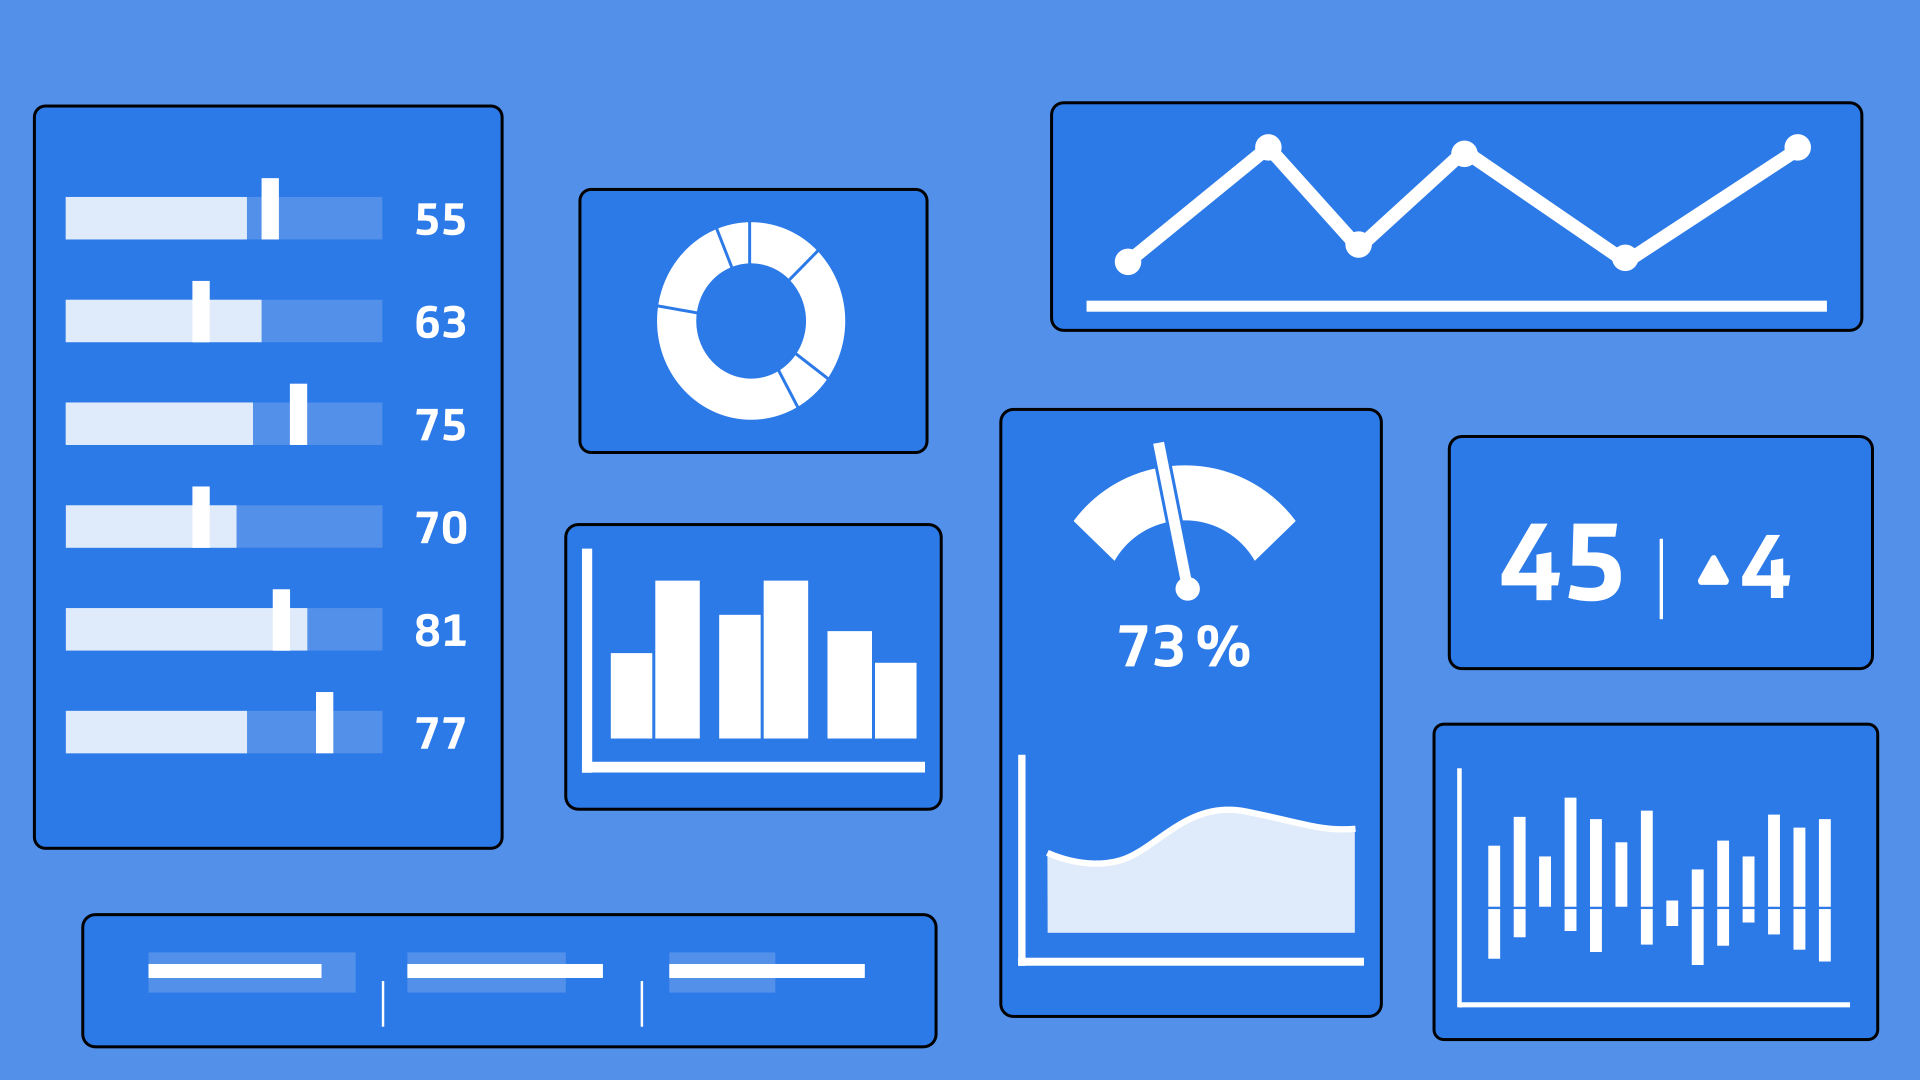
\includegraphics[width=0.80\columnwidth]{immagini/dashboard.png}
    \caption{\textit{Dasboard} - Fonte: \href{https://www.klipfolio.com/resources/articles/what-is-a-key-performance-indicator}{Measure your performance against key business objectives - Klipfolio}}
    \label{fig:my_label}
\end{figure}

%**************************************************************
\section{Il ruolo di Bipod in Siav}
%**************************************************************
\subsection{Prerogative}
Bipod viene continuamente sviluppato per dare valore aggiunto alle soluzioni software Siav. Esso si integra nel concetto di trasformazione digitale proponendosi di coprire sempre più esigenze di consulenti ed amministratori, dalla rilevazione al monitoraggio.

\'E un prodotto completo perché tramite la partizione principale \textit{back-end} rende fruibili i dati contenuti nei registri di processo, offre delle \acrshort{api} per l'inserimento e gestione dei \acrshort{kpi} e infine ne esegue tutte le operazioni di monitoraggio e rilevazione.

La partizione \textit{front-end} si occupa di comunicare le richieste utente al resto dell'applicazione tramite chiamate ad \acrshort{api} e tramite un \textit{websocket} utile allo smaltimento del carico di elaborazione, gestito sempre dal \textit{back-end}. Il suo scopo è quello di permettere tramite interfaccia grafica, di esprimere i corretti comandi da recapitare alla parte software incaricata di gestire le sue richieste.

%**************************************************************
\subsection{ProM - un valido concorrente?}
Con ProM si identifica un framework di sviluppo che permette di estrarre informazioni da un registro di processo. Sviluppato e manutenuto dal \textit{Process Mining Group} dell'università di Eindhoven, viene integrato nella suite software \textit{ProM Tools}. Nel pacchetto software è possibile trovare diversi strumenti per l'ispezione dei processi sia in modalità testuale, sia in modalità grafica.

ProM Tools essendo uno stumento nato dalla ricerca, possiede un interfaccia grafica estremamente basilare ma gode di una completezza nell'analisi dei \textit{log} di processo e maggiore personalizzazione nell'output di grafi e grafici.
%**************************************************************
\subsection{Bipod - uno strumento flessibile}
Lo scopo di Bipod non è quello di creare una copia marchiata Siav dei ProM tools bensì quello di rendere le loro funzionalità più accessibili ed intuitive anche a chi ha un primo approccio a questo tipo di software.
Altra parte dello studio costante che è alla base dello sviluppo dell'applicazione, è quella di aggiungere la funzionalità di creazione e configurazione cruscotti per amministratori: queste sono necessarie per dare la giusta flessibilità di applicazione nel mondo reale che si concretizza in un valore aggiunto palpabile da più clienti che, utilizzando solo una porzione dei servizi Siav, sono ancora ignari del potenziale.

%**************************************************************
\subsection{L'esperienza utente}
\begin{figure}[H]
    \centering
    
\includegraphics[width=0.80\columnwidth]{immagini/uxneeds.png}
    \caption{In cosa consiste l'UX - Fonte: \href{https://www.genetica.marketing/user-experience-di-cosa-si-tratta/}{UX (User eXperience) - Genetica}}
    \label{fig:my_label}
\end{figure}
La mia attività di stage è stata concretizzare le esigenze conferendo la giusta \acrshort{ux} alla piattaforma.

Lo studio individuale che ha preceduto l'analisi dei requisiti, è stato utile ma ritengo che, una volta acquisite le competenze utili alla comprensione del problema, l'unica soluzione, che è anche quella che insieme a responsabile e tutor abbiamo adottato, è quella di porsi come utente e immaginare scenari di utilizzo.

Molte delle idee, infatti, sono nate nel momento in cui, sviluppandone altre, queste entravano in uso.
Per diversi casi d'uso è stato necessario lavorare tramite dei \textit{mock-up} dell'interfaccia grafica usando il \textit{framework} Angular come strumento di test dell'esperienza utente


%**************************************************************
\subsection{La collaborazione con KaizenKey}
Nelle scelte effettuate per progettare la \acrlong{ux}, un grande aiuto è derivato dalla collaborazione con KaizenKey, partner di Siav tramite un rapporto pluriennale di collaborazione. KaizenKey è infatti uno dei primi fruitori della piattaforma Bipod: il sostegno reciproco si basa sulla fiducia che Siav pone in KaizenKey per la loro attività in ambito di analisi e consulenza sui processi aziendali. Proprio per questo, in reparto, ci siamo confrontati con loro, sopratutto nelle prime settimane, facendo nascere nuove idee da sviluppare.

In particolare sono state molto utili alcuni sugeggerimenti riguardo alla definizione di termini e alla visualizzazione di alcune proposte frequentemente usate nell'analisi di processo durante l'accesso al configuratore da parte del consulente.

\begin{figure}[H]
    \centering
    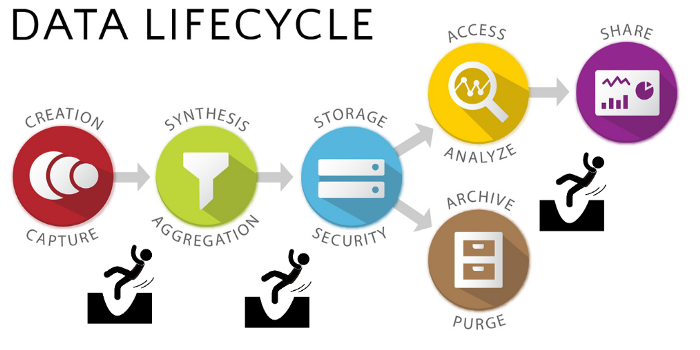
\includegraphics[width=0.80\columnwidth]{immagini/data_lifecycle.png}
    \caption{Ciclo di vita del dato - Fonte: \href{https://medium.com/digital-transformation-in-the-asset-management/from-data-to-insights-the-immediate-pitfalls-part-i-data-creation-collection-7948568c0059}{From data to insights - pt.1 - Medium}}
    \label{fig:my_label}
\end{figure}